\section{Experimentación y Resultados}

Al experimentar siempre es de suma importancia elegir los casos de prueba. Como es un algoritmo que depende de una semilla random lo primero que decidimos fue dejarla fija, para que las sucesivas ejecuciones fuesen de la misma naturaleza. El algoritmo es de complejidad lineal respecto de divisiones por cantidad de picos, por ende al experimentar probamos diferentes combinaciones de los mismos.\\

Basandonos solo en la teoría, en un comienzo suponíamos una mejora en la performance de ASM cercana a 16 veces la de C. Llegamos a ese número partiendo de que, si C no tenía ninguna mejora iba a poseer la complejidad teórica de divisiones por cantidad de picos; mientras que nuestro ASM recorría tanto las divisiones como los picos de a cuatro, si consideramos esto nos queda $divisiones/4 * picos/4$. Esta complejidad es del mismo orden de grado (lineal) modificada solo por la constante $1/16$, presentando así una mejora del 93.75$\%$.\\

Para la recolección de datos utilizamos la librería Nonius\footnote{\url{https://nonius.io/}} que toma varias muestras, corriendolas muchas veces y procesa los resultados eliminando outliers. Las pruebas fueron corridas sobre un procesador Intel$^{®}$ Core™ i5-6200U\footnote{\url{https://ark.intel.com/es-es/products/88193/Intel-Core-i5-6200U-Processor-3M-Cache-up-to-2_80-GHz}}.\\

Los datos con los que fueron generados los gráficos se encuentran la siguiente url \url{http://cor.to/OrgaIIDatos} y los gráficos se encuentran de manera interactiva en las url al pie de la página de cada uno.

\subsection{Misma cantidad de picos, distintas divisiones}
Como primer experimento fijamos la cantidad de picos y fuimos aumentando las divisiones.

\centerline{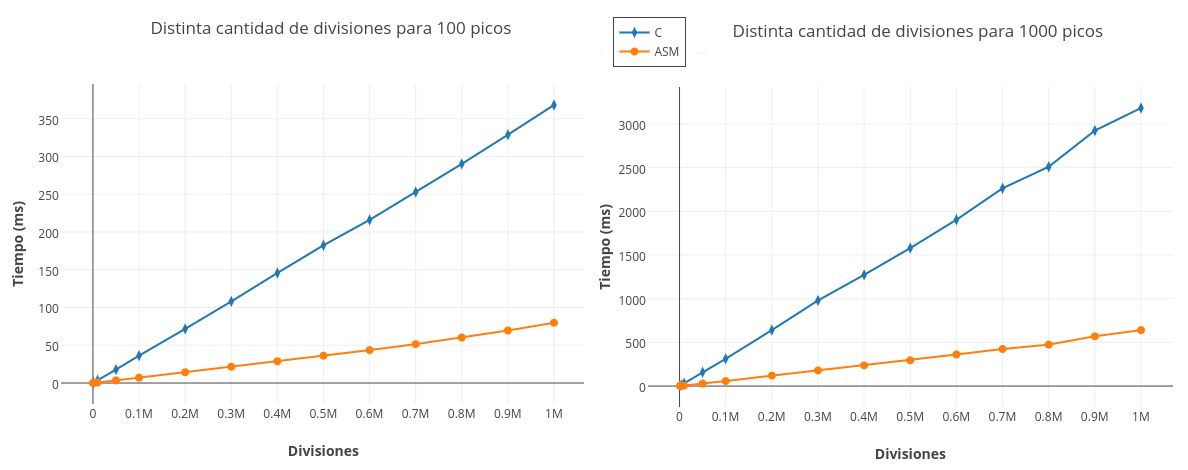
\includegraphics[scale=0.45]{imagenes/distintasDivisionesParaPicos.png}}\footnote{ 100 picos: \url{https://plot.ly/~fzanollo/55/} 1000 picos: \url{https://plot.ly/~fzanollo/53/}} 

En el gráfico de la izquierda probamos con 100 picos, como se ve al aumentar las divisiones el tiempo consumido crece de forma lineal. Si bien se presenta una mejora promedio del 78$\%$, no alcanza a los valores teóricos esperados.

En el de la derecha con 1000 picos. A pesar de que el gráfico muestra la misma tendencia analizando los datos encontramos que ahora la mejora es un poco más notoria y se eleva al 81$\%$.

\newpage

\subsection{Misma cantidad de divisiones, distinto porcentaje de picos}

El siguiente conjunto de casos de prueba fueron con una cantidad fija de divisiones, variando el porcentaje de picos respecto a las mismas.\\

Estos gráficos resultaron muy parecidos entre sí y respecto al anterior conjunto de pruebas. 

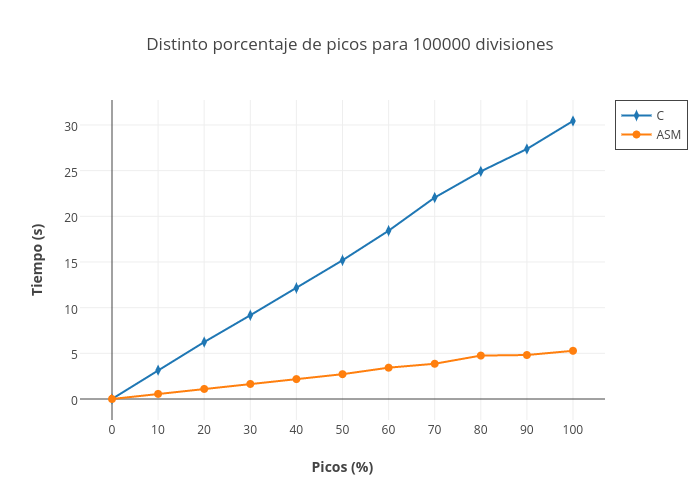
\includegraphics[scale=0.6]{imagenes/distintosPicos100000divisiones.png}\footnote{ 100000 divisiones: \url{https://plot.ly/~fzanollo/51/}}  

A medida que se aumentan las divisiones el gráfico se asemeja más al de una función lineal ya que se obtienen resultados más fehacientes.\\

Esto es porque, normalmente, a la hora de medir cantidad de ciclos de CPU pueden suceder diferentes eventos que alteran las mediciones, el ruido generado por los eventos se notan más si son pocos ciclos.

\centerline{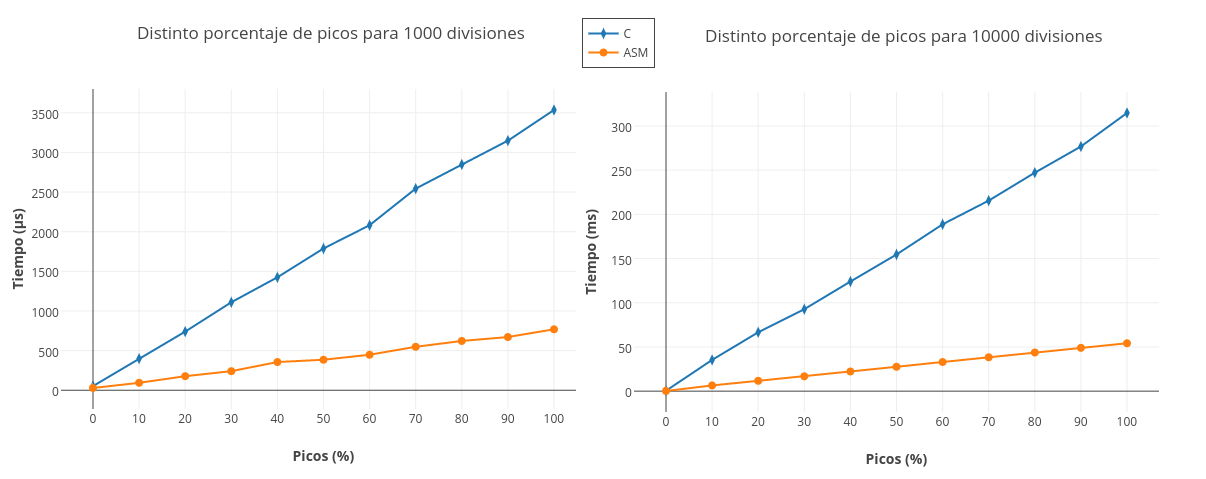
\includegraphics[scale=0.45]{imagenes/distintosPicosParaDivisiones.png}}\footnote{ 1000 divisiones: \url{https://plot.ly/~fzanollo/61/} 10000 divisiones: \url{https://plot.ly/~fzanollo/59/}} 

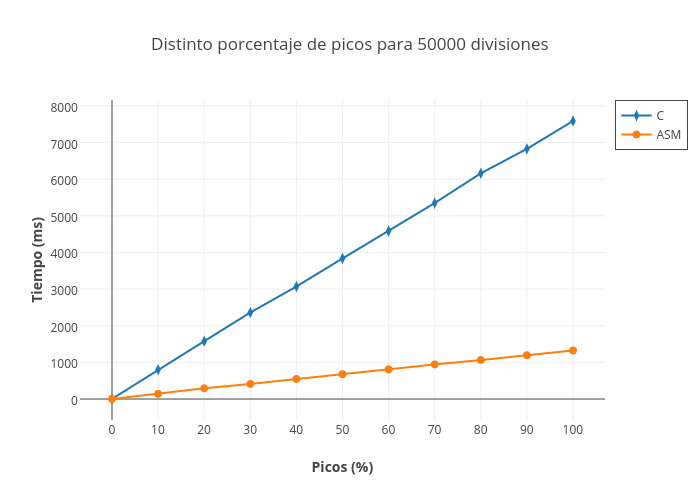
\includegraphics[scale=0.6]{imagenes/distintosPicos50000divisiones.png} \footnote{ 50000 divisiones: \url{https://plot.ly/~fzanollo/57/}} 

Dado que eran muy parecidos decidimos presentar los casos más chicos (1000 y 10000 divisiones) conjuntamente. La mejora promedio aproximada entre todos estos casos de prueba es del 80$\%$.

\newpage
\subsection{Misma cantidad de tamaño de entrada}

En los casos de prueba que listamos previamente mantuvimos fija una variable (cantidad de picos o cantidad de divisiones) e incrementamos la restante, como complemento realizamos un análisis manteniendo el tamaño total fijo, lógicamente la cantidad de picos no puede superar a la de divisiones.
Cantidad de picos p x Cantidad de divisiones d = Tamaño de entrada total T

En principio pensamos que el tiempo de ejecución debería mantenerse en todos los casos, debido a que tienen la misma complejidad teórica. En todo caso aumentando ligeramente para los casos con mayor cantidad de picos, debido a los cálculos previos para obtener los datos aleatorios de las ubicaciones y tamaños.

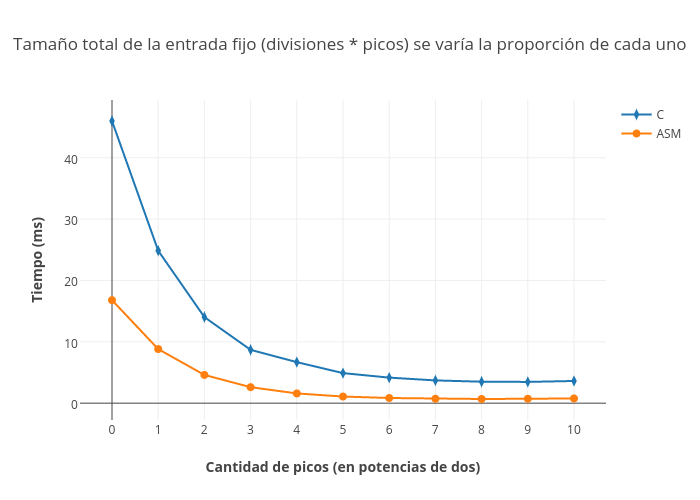
\includegraphics[scale=0.6]{imagenes/tamanioTotalFijo.png} \footnote{ Tamaño total fijo: \url{https://plot.ly/~fzanollo/63/}} 

Como vemos en el gráfico, a medida que crece el número de picos y disminuye la cantidad de divisiones, el tiempo de procesamiento decrece.\\

Obtuvimos un grupo de casos, desde un pico con 1024x1024 divisiones hasta 8 picos con 1024x128 divisiones (en el gráfico desde 0 hasta 3), que presenta un comportamiento diferente al resto en cuanto a tiempo de procesamiento.

Si bien estos casos podrían analizarse en profundidad, vamos a descartarlos ya que poseen un porcentaje de picos muy bajos para una generación de terreno concreta (mucho menos del 1$\%$).\\

Para el resto de los casos donde los porcentajes de picos sobre divisiones son más considerables, las gráficas se observan más estables.